% !TEX TS-program = pdflatex
% !TEX encoding = UTF-8 Unicode

\documentclass[a4paper]{report}

\usepackage[english]{babel}
\usepackage[T1]{fontenc}
\usepackage[utf8]{inputenc}
\usepackage[pdftex]{graphicx}
\usepackage{float}
\usepackage{fancyhdr}
\usepackage[toc,page]{appendix}
\usepackage{listings}
\usepackage{booktabs} % for much better looking tables
\usepackage{array} % for better arrays (e.g. matrices) in maths
\usepackage{paralist} % very flexible & customizable lists (e.g. enumerate, etc.)
\usepackage{verbatim} % adds environment for commenting out blocks of text & for better verbatim
\usepackage{subfig} % make it possible to include more than one captioned figure / table in a single float
\usepackage[margin=2.5cm]{geometry}

\usepackage{titling} % for useful adjustments to the titles
\usepackage[hyphens]{url} % for simple URL formatting
\usepackage[numbers,sort]{natbib} % automatic short-hand citations

\usepackage[plain]{fancyref} % auto-detection of cross-referenced types
\usepackage{listings} % code listings
\usepackage{shortvrb} % shorthand pre-formatted text

\usepackage{hyperref} % useful stuff for references
\usepackage[hypcap]{caption} % smarter pointing for reference links

\usepackage[nottoc,notlof,notlot]{tocbibind} % Put the bibliography in the ToC
\usepackage{multicol}

\setlength{\parindent}{0pt}

%%% Headers, footers
\author{Niclas Olofsson}
\pagestyle{fancy}
\renewcommand{\headrulewidth}{1pt}
\fancyhead[LO,L]{Automated testing of a dynamic web application}
\lfoot{}\cfoot{\thepage}\rfoot{}

%%% Custom chapter and section style
\usepackage{titlesec, blindtext, color}
\definecolor{gray75}{gray}{0.75}
\newcommand{\hsp}{\hspace{20pt}}

\usepackage{sectsty}
\allsectionsfont{\sffamily\mdseries\upshape} % sans serif headings

\newcommand{\quotes}[1]{``#1''}

\titleformat{\chapter}[hang]{\Huge\bfseries}{\thechapter\hsp\textcolor{gray75}{|}\hsp}{0pt}{\Huge\bfseries}

\lstset{
language=Ruby,
basicstyle=\small\sffamily,
numbers=left,
numberstyle=\tiny,
frame=tb,
columns=fullflexible,
showstringspaces=false
}

%%% Title page
\makeatletter
\newcommand{\myinfo}{
  \gdef\@myinfo{%
  \begin{tabular}{cl}
  Supervisor & Anders Fröberg\\
             & IDA, Linköping University\\
  \\
  Examiner & Erik Berglund\\
           & IDA, Linköping University\\
  \\
  Technical  & Mattias Ekberg\\
  supervisor & GOLI AB\\
  \end{tabular}
  \par\vspace{12pt}
  \textsc{Linköping University\\
          Department of Computer and Information Science}}
}
% add the extra information after the date
\postdate{\par\vspace{12pt}\@myinfo\end{center}}
\makeatother

\title{\textsc{Final thesis}\\\Huge\textbf{Automated testing of a dynamic web application}}
\author{Niclas Olofsson}
\date{\today}

\myinfo

\begin{document}

\renewcommand{\lstlistingname}{Code listing}

\maketitle
\newpage

\begin{abstract}
Software testing plays an important role in the process of verifying
software functionality and preventing bugs in production code. By
writing automated tests using code instead of conducting manual tests,
the amount of tedious work during the development process can be reduced
and the software quality can be improved.\\

This thesis presents the results of a conducted case study on how
automated testing can be used when implementing new functionality in a
Ruby on Rails web application. Different frameworks for automated
software testing are used as well as test-driven development
methodology, with the purpose of getting a broad perspective on the
subject. This thesis studies common issues with testing in these kinds of
applications, and discuss drawbacks and advantages of different testing
approaches. It also looks into quality factors that are applicable for
tests, and analyze how these can be measured.\\

\end{abstract}

% Fake that the Acknowledgments is an abstract in order to get a nice style
\renewcommand{\abstractname}{Acknowledgments}

\begin{abstract}
This final thesis was conducted at GOLI AB, on the business incubator
LEAD during the spring of 2014. I would like to thank my dear colleagues
Lina, Malin and Madeleine, as well as all other people at LEAD for good
fellowship and encouragement during this period. I specially want to
thank my technical supervisor Mattias for help, support, interesting
discussions and ideas.\\

I would also like to give thanks to my supervisor Anders Fröberg for
help with finding and narrowing down the problem formulation, and my
examiner Erik Berglund for overall help and support.\\

\end{abstract}

\setcounter{tocdepth}{4}
\tableofcontents
\thispagestyle{empty} % No page numbering of ToC pages
\newpage

\setcounter{page}{1}

\chapter{Introduction}

  \section{Background}
  \label{sec:background}
  During code refactoring or implementation of new features in software,
errors often occur in existing parts. This may have a serious impact on
the reliability of the system, thus jeopardizing user's confidence for
the system. Automatic testing is utilized to verify the functionality of
software in order to detect bugs and errors before they end up in a
production environment.\\

Starting new web application companies often means rapid product
development in order to create the product itself, while maintenance
levels are low and the quality of the application is still easy to
assure by manual testing. As the application and the number of users
grows, maintenance and bug fixing becomes an increasing part of the
development. The size of the application might make it implausible to
test in a satisfying way by manual testing.\\

The commissioner body of this project, GOLI, is a startup company
developing a web application for production planning called GOLI
Kapacitetsplanering. Due to requirements from customers, the company
wishes to extend the application to include new features for handling
staff manning. The current system uses automatic testing to some extent,
but these tests are cumbersome to write and takes long time to run. The
purpose of the thesis is to analyze how this application can begin using
tests in a good way whilst the application is still quite small. The
goal is to determine a solid way of implementing new features and bug
fixes in order for the product to be able to grow effortlessly.\\


  \section{Problem formulation}
  
The goal of this final thesis is to analyze how automated tests can be
introduced in an existing web application, in order to detect software
bugs and errors before they end up in a production environment. In order
to do this, a case study is conducted. The focus of the case study is
how automated testing can be done in the specific application. The
results from the case study are used for discussing how testing can be
applied to dynamic web applications in general.\\

The main research question is to determine how testing can be introduced
in the scope of the application. Which tools and frameworks are
available, and how well do they work in the given environment? How can
test-driven development methodologies be used and how can we evaluate
the quality of the written tests? The research is focused on techniques
which are relevant the specific application, i.e. techniques relevant
to web applications that uses Ruby on
Rails\footnote{\url{http://rubyonrails.org/}} and
KnockoutJS\footnote{\url{http://knockoutjs.com/}} with a
MongoDB\footnote{\url{https://www.mongodb.org/}} database system for
data storage.\\


  \section{Scope and limitations}
  There exists different categories of software testing, for example
performance testing and security testing. The scope of this thesis is
tests in which the purpose is to verify the functionality of a part of
the system rather than measuring its characteristics. We will also only
cover automatic testing, as opposed to manual testing where the
execution and result evaluation of the test is done by a human. The term
\emph{testing} will hereby refer to automatic software testing unless
specified otherwise.\\

We will also not cover testing static views or any issues related to the
deployment of a dynamic web application, but rather testing of the
dynamic application itself.


  \section{Conventions and intended audience}
  \MakeShortVerb{\|}

\subsection{Writing conventions}

Terms written in \emph{italics} are subjects that occur further on in
this thesis. Understanding the meaning of these may be required for
understanding concepts later on.\\


\subsection{Choices and definitions}

Code examples are written in Ruby\footnote{\url{https://www.ruby-
lang.org}} 2.1.1 since that is the primary language of this project. The
focus of the code examples is yet to be understandable by people without
knowledge of Ruby, rather than using Ruby-specific practices. For
example, implicit |return|-statements are avoided since these are
hard to understand for people used to languages without this feature,
such as Python or Java. Code examples typically originate from
implemented code, but names of classes and functions have been altered
for copyright, consistency and understandability reasons.\\

The built-in Ruby module Test::Unit is used for general test code
examples in order to preserve the independence of a specific testing
framework as far as possible, although other testing frameworks are also
mentioned and exemplified in this thesis. Another reason for this choice
is to avoid introducing unnecessary complexity for these examples.\\

The area of software development contains several terminologies that are
similar or exactly the same. In cases where multiple different
terminologies exist for a certain concept, we have chosen the term with
most hits on Google. The purpose of this was to choose the most widely-
used term, and the number of search results seemed like a good measure
for this. A footnote with alternative terminologies is present when
such terminology is defined.\\

The term \emph{testing} will in this report refer to automatic software
testing with the purpose of finding software defects, unless specified
otherwise. We will also refer to the GOLI Kapacitetsplanering software
as \emph{the application}. We will use the term \emph{test-driven
development methodologies} as a collective term for both test- and
behavioral driven development (explained in \fref{sec:tdd} and
\ref{sec:bdd}).\\



\chapter{Methodology}
  
This chapter outlines the general research methodology of this thesis,
and explains how different choices was made.\\

\section{Introduction}
The methodology of this thesis is generally based on the guidelines
proposed by \citet{article:casestudies} for conducting a case study.
An objective is defined and a literature study is conducted in
order to establish a theoretical base. The theory is then evaluated by
applying it in a real-life application context, and the result is
analyzed in order to draw conclusions about the theory.


  \section{Literature study}
  
The literature study is based on the problem formulation, and therefore
focus on web application testing overall and how it can be automated. In
order to get a diverse and comprehensive view on these topics, multiple
different kinds of sources were consulted. As a complement to a
traditional literature study of peer-reviewed articles and books, we
have also chosen to also consider blogs and video recordings of talks
from developer conferences.\\

While blogs are neither published nor peer-reviewed, they often express
interesting thoughts and ideas, and often give readers a chance to leave
comments and discuss its contents. This might not qualify as a review
for a scientific publication, but it give readers larger possibilities
of leaving feedback on outdated information and fact errors. It also
makes it possible to discuss the subject to a larger extent and give
additional views on the subject.\\

Recordings of people speaking at developer conferences have similar
properties when it comes to their content, lack of reviewing process and
greater possibilities for discussion. One benefit is however that speakers
at such conferences tend to be experts on their subjects, which might
not be the case for a majority of all people writing blogs.\\

Blogs and talks from developer conferences have another benefit
over articles and books since they can be published instantly. The
review- and publication process for articles is long and may take
several months, and might also fail to be available in online databases
until after their embargo period has passed \cite{wiki:embargo,
pdf:publishing}. This can make it hard to publish up-to-date scientific
articles about some web development topics, since the most recent
releases of commonly used web frameworks are less than a year old
\cite{wiki:rails_versions, wiki:django_versions,
web:knockout_versions}.\\

Utilized alternative sources are mainly relied upon recognized people in
the open-source software community. One main reason for this is that
large parts of the web development community as well as the Ruby
community are pretty oriented around open-source software and agile
approaches. This is also the case for several test-driven techniques and
methodologies. Due to this, one might notice a tilt in this thesis
towards agile approaches and best practices used by the open-source
community.\\


  \section{Choices of technologies and frameworks}
  \MakeShortVerb{\|}
\label{sec:choices}

The choice of frameworks for development was mainly given by the
constituent, since the existing software was written in Ruby on Rails
with KnockoutJS and a MongoDB database. The main server-side language
was thus Ruby, and the client-side code was written in CoffeeScript.
CoffeeScript is a scripting language which compiles into Javascript.\\

For the choice of testing-related frameworks, we choose to look for
frequently used and active developed open source frameworks.
Technologies that are used by many people intuitively often has more
resources on how they are used, and also has the advantage of being more
likely to be recognized by future developers. Active development of used
frameworks is crucial, most importantly since they are likely to be
incompatible with future versions of other frameworks (such as Rails).
Another benefit is that new features and bug fixes are released.\\

The Ruby Toolbox website \footnote{\url{https://www.ruby-toolbox.com/}},
which uses information from the Github and RubyGems websites was
consulted in order to find frameworks with mentioned qualities.\\

\subsection{Ruby test frameworks}
RSpec, RSpec-mocks, Cucumber, Capybara, FactoryGirl, Timecop, site\_prism. (wip)


\subsection{Javascript test frameworks}

There exists a few different frameworks for testing Javascript or
CoffeeScript code. We had previously good experiences from working with
Jasmine\footnote{\url{http://jasmine.github.io/}}. We also found that
this framework seemed to be very popular, actively developed and had
good documentation\footnote{It is worth to mention that the Jasmine
documentation is basically its own test suite with some additional
comments. This works incredibly good in this case, presumably since it
is a test framework.}. Its syntax is inspired by RSpec, which also is an
advantage since RSpec is used for the server side tests.\\

The Jasmine framework provides a way of writing tests, but a test runner
is also required in order to run the tests. Jasmine ships with a basic
test runner which was used initially, which worked out-of-the box using
the Jasmine Ruby gem. A screenshot of this test runner is shown in
\fref{fig:jasmine_runner}.\\

\begin{figure}
\centering
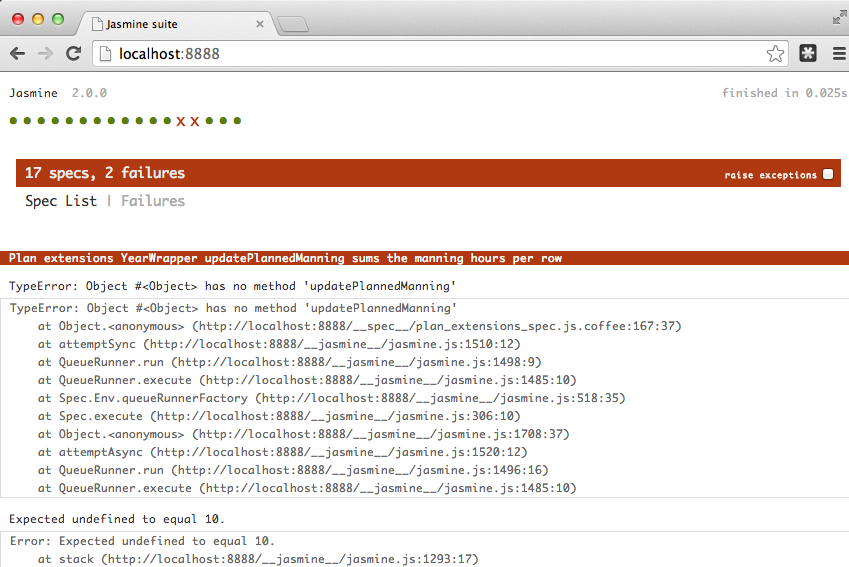
\includegraphics[width=0.8\textwidth]{methodology/jasmine_runner}
\caption{The test runner bundled with Jasmine.}
\label{fig:jasmine_runner}
\end{figure}

The Jasmine test runner did however have multiple issues. First of all,
it runs completely in the browser. Switching to the browser and reload
in order to run the tests are not excessively problematic, but might be
a little bit tiresome in the long run when using a test-driven
development methodology. A larger problem was the fact that the asset
handling, i.e. the compilation of CoffeeScript into Javascript, is
handled by Rails upon each reload. Rails currently re-compiles all
assets upon page load if any file has been changed. This process takes a
while, which means that each test run could take up to 10-15 seconds
even though the actual tests only takes a fraction of a second to run.
The asset compilation also got stuck for for apparently no reason once
in a while. Since the server port on which the test runner runs cannot
be specified, it is also impossible to restart the test runner without
manually killing its process.\\

Due to these issues, we switched to the Karma\footnote{\url{http
://karma-runner.github.io/}} test runner. Karma originates from a
master's thesis by \citet{article:karma}, and this thesis also covers
several problems with other test runners (such as the mentioned Jasmine
test runner). Karma was designed to solve several of these issues and to
be used with test-driven software methodologies. Test are run in a
browser as soon as a file is changed, and the results are reported back
to the terminal and displayed as shown in \fref{fig:karma_runner}.\\

\begin{figure}
\centering
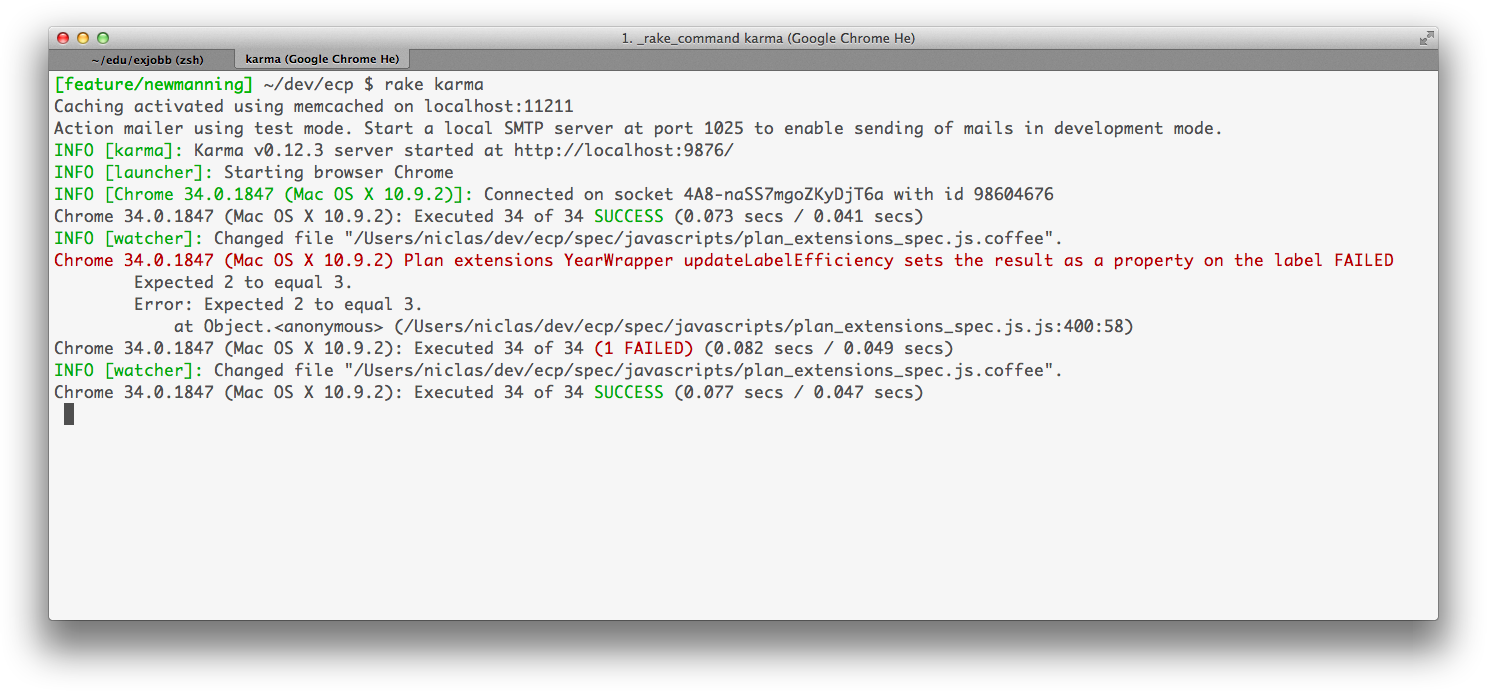
\includegraphics[width=0.8\textwidth]{methodology/karma_runner}
\caption{The Karma test runner.}
\label{fig:karma_runner}
\end{figure}

\subsection{Test coverage}
\label{sec:coverage_frameworks}

\subsubsection{Ruby test coverage}
There are multiple different ways of analyzing test coverage, and the
properties and conditions for each different kind of test coverage are
discoursed in \fref{sec:coverage}. However, we were unable to find any
test coverage tools for Ruby which analyzed anything else than statement
coverage, which is the weakest test coverage metric. Quite much effort
was spent on finding such tool, but without any success. Several
websites and Stack Overflow-answers indicates that no such tool exists
for Ruby at the time of this writing \cite{web:coverage_ruby19,
so:c1c2_coverage, so:c1_coverage, web:toolbox_code_metrics}. On one
hand, some of these sources are rather old and might be outdated, which
would indicate that such tool could have been created recently. On the
other hand would at least some of these sources probably been updated if
such tool became available.\\

We ended up using the
SimpleCov\footnote{\url{https://github.com/colszowka/simplecov}} tool
for Ruby test coverage metrics. At the time of this writing, it is the
most used Ruby tool for test coverage. It is also actively developed,
works with recent Ruby versions and RSpec versions, and produces pretty
and easy- to-read coverage reports in HTML (see
\fref{fig:simplecov_report}).\cite{web:toolbox_code_metrics}\\

\begin{figure}
\centering
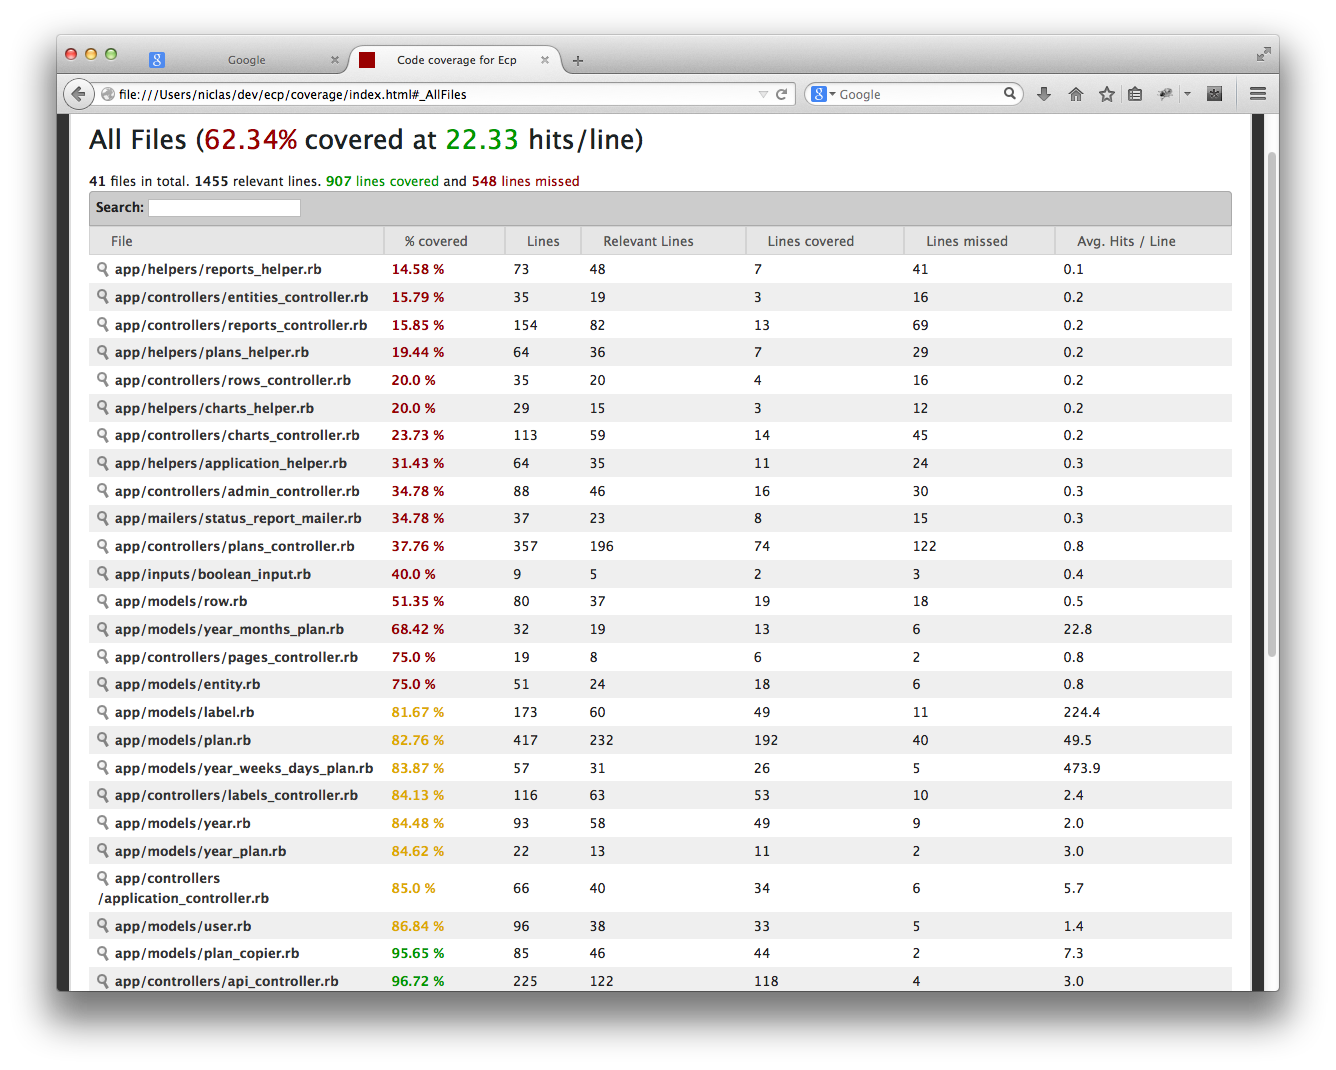
\includegraphics[width=0.8\textwidth]{results/simplecov}
\caption{A coverage report generated by SimpleCov}
\label{fig:simplecov_report}
\end{figure}

\subsubsection{CoffeeScript test coverage}
For the client-side CoffeeScript, we used a plug-in for the Karma test
runner called karma-coverage\footnote{\url{https://github.com/karma-
runner/karma-coverage}}. This tool basically integrates Karma with
Ibrik\footnote{\url{https://github.com/Constellation/ibrik}}, which is a
tool developed by Yahoo! for measuring test coverage of CoffeeScript
code. We did initially have some problems with getting this tool to work
correctly, since Ibrik internally uses another CoffeeScript compiler;
CoffeeScriptRedux, than the compiler used when tests itself are run.
CoffeeScriptRedux is more strict and yielded syntax errors in some of
our files, which could be compiled correctly in the production code. The
latest available release of Ibrik (version 1.1.1) also had major issues
with certain constructs in CoffeeScript, which made the files impossible
to analyze. This issues was however fixed in the development version.
Ibrik was first released in December 2013, which may explain its
immaturity. Ibrik internally uses istanbul-js for the coverage
analysis and report generation.\\

The chosen solution worked very well after sorting out the issues.
Statement coverage as well as branch coverage is supported, and it
yields useful reports. As with SimpleCov, the coverage reports are
produced as an interactive HTML report (see \fref{fig:karma_report}).\\

\begin{figure}
\centering
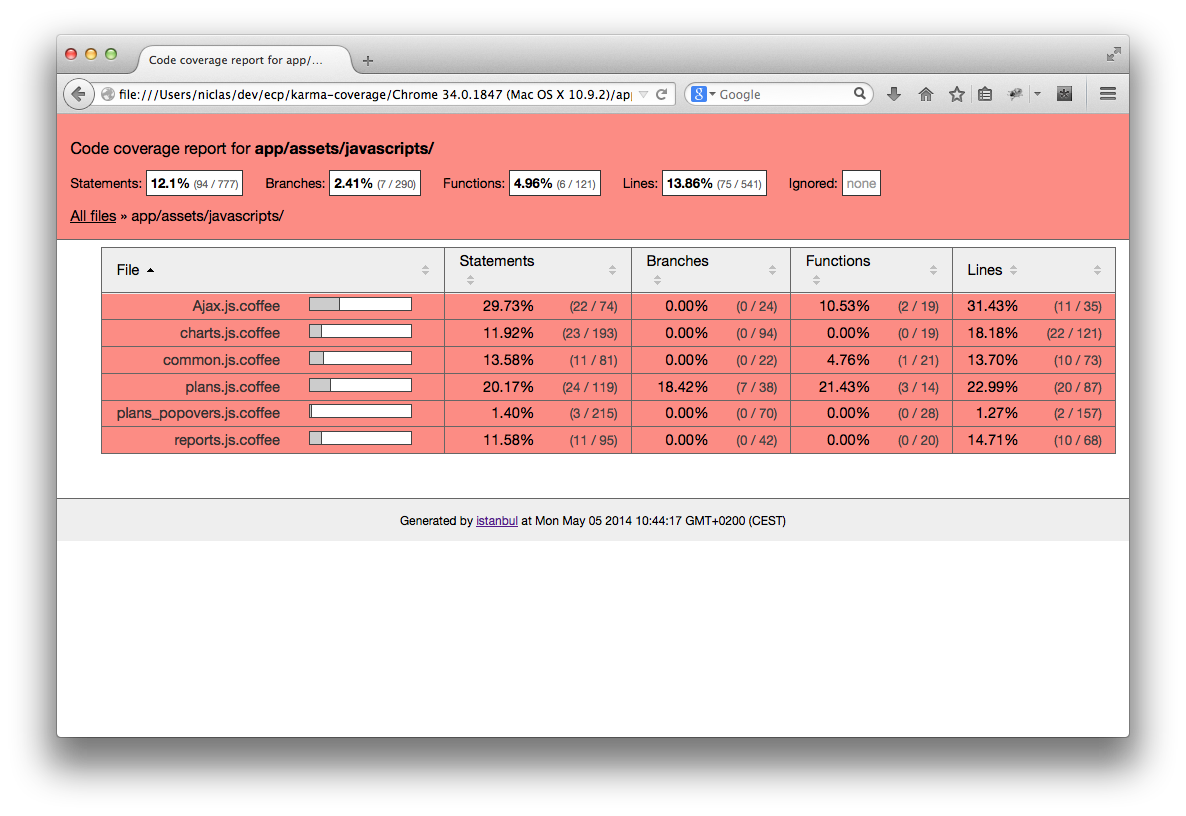
\includegraphics[width=0.8\textwidth]{methodology/karma_coverage}
\caption{A coverage report generated by istanbul-js using karma-coverage}
\label{fig:karma_report}
\end{figure}

\subsubsection{Test coverage issues}

One issue with using test coverage in this particular project is the
fact that very few files were added. Most of the changes was made in
existing classes and files, either as new functions or as changes to
existing functions. Since the overall test coverage is measured per
file, it is impossible to get an exact measure of how well-tested the
new and re-factored code is, since old and completely untested code
lower the test coverage.\\

We have tried to mitigate this by looking at the coverage reports by
hand, and try to determine a subjective measure of how good the test
coverage is for new and re-factored code. \Fref{fig:coverage_example}
shows an excerpt of a coverage report. In this case, our subjective
measure would say that the function |exports.getProduction()| is
completely untested. The function |exports.getLabelId()| is well tested
and has full statement- as well as branch coverage. The function
|exports.formatValues()| has full statement coverage, but non-optimal
branch coverage since the cases where |x| or |y| is not set are not
covered.\\

\begin{figure}
\centering
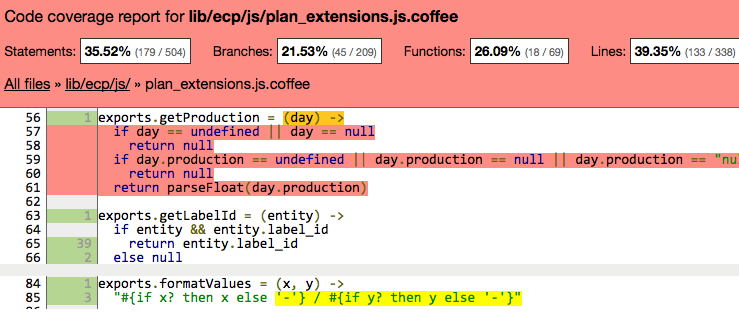
\includegraphics[width=0.8\textwidth]{results/js_coverage}
\caption{An excerpt from a coverage report generated using karma-coverage
         which demonstrates three different types of tested functions.}
\label{fig:coverage_example}
\end{figure}

\subsection{Mutation analysis}
\label{sec:choices_mutation}

There exists a few different tools for mutation analysis of Javascript
code. The ones we have found originates from academic research papers.
\citet{paper:mutandis} proposes a solution which has been implemented as
a tool called Mutandis
\footnote{\url{https://github.com/saltlab/mutandis/}}.
\citet{paper:ajaxmutator} presents another approach which has been
released as AjaxMutator \footnote{\url{https://github.com/knishiura-
lab/AjaxMutator}}. \citet{paper:webmujava} proposes a system-level
mutation testing approach called webMuJava.\\

Mutandis is based on website crawling tests. Although
\citeauthor{paper:mutandis} mentions that pure Javascript frameworks
have been tested using this tool, its implementation showed to be too
specific to be considered in our context. webMuJava does not seem to be
publicly available, and also seems to be too tightly integrated with a
specific back-end technique to be useful for Javascript-testing only.

AjaxMutator is in our opinion the most mature of all the considered
frameworks. It provides some basic documentation and installation
instructions, and the amount of implementation needed in order to begin
using it in a new project is reasonable. However, AjaxMutator currently
only supports Javascript tests written in Java using
JUnit\footnote{\url{http://junit.org/}}. Using it for mutation testing
tests written in CoffeeScript using Jasmine would probably be possible,
but the effort of doing this is outside the scope of this thesis.\\



  \chapter{Theory}
  \label{chap:theory}

  \section{Levels of testing}

    \subsection{Unit-testing}
    \label{sec:unit_testing}
    \MakeShortVerb{\|}

% In order to verify the functionality of program, it is possible to use a
% formal logical proof. This is done dividing the program into small
% pieces of logic, and the possible input data into different classes.
% \citet{book:pfleeger}

Unit testing\footnote{Also called low-level testing, module testing or
component testing} refers to testing of small parts of a software. In
practice, this often means testing a specific class or method of a
software. The purpose of unit tests is to verify the implementation,
i.e. to make sure that the tested unit works correct
\cite{book:pfleeger}.\\

Since each unit test only covers a small part of the software, it is
easy to find the cause for a failing test. Writing unit tests alone does
not give a sufficient test coverage for the whole system, since unit
tests only assures that each single tested module works as expected. A
well- tested function for validating a 12-digit personal identification
number is worth nothing if the module that uses it passes a 10-digit
number as input \cite{wiki:unittests}.\\


\subsubsection{Testability}

Writing unit tests might be really hard or really easy depending on the
implementation of the tested unit. \citet{video:misko_psychology} claims
that it is impossible to apply tests as some kind of magic after the
implementation is done. He demonstrates this by showing an example of
code written without tests in mind, and points out which parts of the
implementation that makes it hard to unit-test.
\citeauthor{video:misko_psychology} mentions global state variables,
violations of the Law of Demeter, global time references
and hard-coded dependencies as some causes for making implementations
hard to test.\\

Global states infers a requirement on the order the tests
must be run in, which is bad since it is often non-deterministic and
therefore might change between test runs. Global time references is bad
since it depends on the time when the tests are run, which means that a
test might pass if it is run today, but fail if it is run tomorrow.\\

The Law of Demeter\footnote{Also called the principle of least
knowledge} means that one unit should only have limited knowledge of
other units, and only communicate with related modules
\cite{wiki:demeter}. If this principle is not followed, it is hard to
create an isolated test for a unit which does not depend on unrelated
changes in some other module. The same thing also applies to the usage
of hard-coded dependencies. This makes the unit dependent on other
modules, and makes it impossible to replace the other unit in order to
make it easier to test.\\

\citeauthor{video:misko_psychology} shows how code with these issues can
be solved by using dependency injection and method parameters instead
of global states and hard-coded dependencies. This makes testing of the
unit much easier.\\


\subsubsection{Stubs, mocks and factory objects}
\label{sec:theory_mocks}

Another way of dealing with dependencies on other modules is to use some
kind of object that replaces the other module. The replacement object
has a known value that is specified in the test, which means that
changes to the real object will not affect the test. The reasons for
using replacement objects is often to make it more robust to code
changes outside the tested unit. It might also be used instead of calls
to external services such as web-based API:s in order to make the tests
run when the service is unavailable, or to be able to test
implementations that depends on classes that has not been yet.\\

The naming of different kinds of replacement objects may differ, but two
often used concepts are \emph{stubs} and \emph{mocks}. Both these
replacement objects are used by the tested unit instead of some other
module, but mocks sets expectations on how it can be used by the tested
module on beforehand. \cite{web:mocks_arent_stubs}\\

Another type of replacement object are \emph{factory objects} or
\emph{fakes}. This kind of object is typically provides a real
implementation of the object that it replaces, as opposed to a stub or
mock which only has just as many methods or properties that is needed
for the test to run. The difference between a fake object and the real
object is typically that fake objects uses some shortcut which does not
work in production. One example is objects that are stored in memory
instead of in a real database, in order to gain performance.
\cite{web:mocks_arent_stubs}\\

\citet{video:boundaries} mentions some of the drawbacks with using mocks
and stubs. If the interface of the replaced unit changes, this might not
be noticed in our test. Consider the scenario given in \ref{lst:mocks}.
In this example we have written a test for the |take_cookie()| method of
the |CookieJar| class, which replaces the |eat_cookie()| method with a
stub in order to make the |CookieJar| class independent of the |Cookie|
class.\\

If we rename the |eat_cookie()| method to |eat()| without changing the
test or the implementation of |take_cookie()|, the test might still pass
although the code will fail in a production environment. This is since
we have mocked an object which no longer exists in the |Cookie| class.\\

Some testing frameworks and plug-ins detects replacement of non-existing
methods and warns or makes the test fail if such mocks are created
\cite{video:boundaries}. Another possible solution is to re-factor the
code to avoid the need for mocks or stubs.\\

\begin{lstlisting}[caption=Example of how mocking might make tests unaware
                           of changes which breaks functionality.,
                   label=lst:mocks, float=t]
class Cookie
    def eat_cookie
        return "Cookie is being eaten"
    end
end

class CookieJar
    def take_cookie
        self.cookies.first.eat_cookie()
        return "One cookie in the jar was eaten"
    end
end

def test_cookie_jar
    Cookie.eat_cookie = Mock
    assert CookieJar.new.take_cookie() == "One cookie in the jar was eaten"
end
\end{lstlisting}


    \subsection{Integration-testing}
    \label{sec:integration_testing}
    Since a unit test only assures that a single unit works as expected,
faults may still reside in how the units works together. The purpose of
integration testing is to test several individual units together, in
order to see if they still work together as intended.\\

There are several ways of performing integration testing, as well as
arguments and opinions about the different ways. \citet{book:adp} state
that integration tests should be built incrementally by extending unit
tests. The unit tests are extended and merged so that they span over
multiple units. The scope of the tests is increased gradually, and both
valid and invalid data is given into the integration tested system unit
in order to test the interfaces between smaller units. Since this
process is done gradually, it is possible to see which parts of the
integrated unit that is faulty by examining which parts have been
integrated since the latest test run.\\

\citet{book:pfleeger} refer to the type of integration testing described
by \citeauthor{book:adp} as \emph{bottom-up testing}, since several
low-level modules (modules at the bottom level of the software) are
integrated into higher-level modules. Multiple other integration
approaches such as \emph{top-down testing} and \emph{sandwich testing}
are also mentioned, and the difference between the approaches is in which
order the units are integrated.\\

\citet{video:integrated_scam} criticizes one kind of integration tests,
which he refers to as \emph{integrated tests}. This refers to
integration tests that are testing the functionality of multiple units
in the same way as unit tests, i.e. by input data and examine the
output. When testing multiple units in this way, one loses the ability
to see which part of all the tested units that are actually failing. As
the number of tested units rises, the number of possible paths will grow
exponentially. This makes it hard to see the reason for a failed test,
but also makes it very hard to decide which of all this paths that needs
to be tested. \citeauthor{video:integrated_scam} claims that this fact
makes developers sloppier, which increases the risk of introducing
mistakes that goes unnoticed through the test suite. If the problem is
solved by writing even more integration tests, developers have less time
to do proper unit tests and instead introduce more sloppy designs. One
may however argue that this argument is based on the fact that
integrated tests to a large part are used instead of unit tests, rather
than as a complement as suggested by \citeauthor{book:pfleeger} and
\citeauthor{book:adp}.\\

Instead of integrated tests, another type of integration tests called
contract- and collaboration tests are proposed. The purpose of these
tests is to verify the interface between all unit-tested modules by
using mocks to test that Unit A tries to invoke the expected methods on
Unit B (contract test). In order to avoid errors due to mocking, tests
are also needed to make sure that Unit B really responds to the calls
that are expected to be performed by Unit A in the contract test. The
idea of this is to build a chain of trust inside our own software via
transitivity. This means that if Unit A and Unit B works together as
expected, and Unit B and Unit C also works together as expected, Unit A
and Unit C will also work together as expected.\\


    \subsection{System-testing}
    System testing is conducted on the whole, integrated software system.
Its purpose is to test if the end product fulfills specified
requirements, which includes determining whether all software units (and
hardware units, if any) are properly integrated with each other. In some
situations, parameters such as reliability, security and usability is
tested.\cite{book:adp}\\

The most relevant part of system testing for the scope of this thesis is
functional testing. The purpose of this is to verify the functional
requirements of the application at the highest level of abstraction. In
other words, one wants to make sure that the functionality used by the
end-users works as expected. This might be the first time where all
system components are tested together, and also the first time the
system is tested on multiple platforms. Because of this, some types of
software defects may never show up until system testing is
performed.\cite{book:adp}\\

\citeauthor{book:adp} proposes that system testing should be performed
as black box tests corresponding to different application use-cases. An
example could be testing the functionality of an online library catalog
by adding a new user to the system, log in and perform different types
of searches in the catalog. Domain-testing techniques such as boundary-
value testing are used in order to narrow down the number of test
cases.\\



  \section{Test methodologies}
    \subsection{Test-driven development}
    \label{sec:tdd}
    
I have striven for using test- and behavioral-driven development
methodologies in the strictest possible way throughout this entire
thesis. The purpose of this has been to gain experience of different
advantages and drawbacks of these methodologies. In situations where I
have found these methodologies to be unsuitable, I have however chosen
to disregard some principles of these methodologies rather than try to
apply them anyway.\\

Using a test-driven approach has two major advantages in our opinion.
The most important is perhaps that it alleviates a sense of fear about
whether or not the implementation really works as it is supposed to, and
a fear that things may break when the code is refactored. The second
important aspect is that the written code is self-testing; one can run a
command in order to find out whether or not the code is in a working
state, rather than testing it manually and see what happens. In
particular, I found writing a failing test before fixing a software
defect to be especially helpful. One can instantly see when the defect
was fixed and therefore know when the work is done, and do not have to
constantly test the software manually during development.\\

Another benefit from using the test-first principle is that one often
think through the design before the implementation. The implementation
has to be written in such way that it is testable, which makes the
developer discover new ways of solving the problem and design the
software better. In some cases this also reduces the amount of written
code since we strive to minimize the number of cases that we have to
test. Additionally, I personally find it tedious to write tests after
the implementation is done. My opinion is that writing the tests first
makes the development more fun than writing tests after
implementation.\\

There is however no guarantee that a more testable design is better than
a less testable design. For example, making it possible to test a
module may require using of a large amount of fake objects such as
mocks. It might also be required to split up the module into several sub
modules that does not map very well to the real world and thus are
difficult to understand. I believe that it is better to test on a
higher level and perhaps discard the test-first principle in cases where
making the code testable introduces more drawbacks than advantages to
the overall design.\\

My main difficulty while using TDD was the \emph{refactor}-part of the
\emph{Red, green, refactor} mantra. I found it hard to know whether or
not code needed to be refactored, and to know how large part of the code
to refactor. Some small changes required large parts of the code to be
refactored in order for the code to be possible to unit-test. In some
situations I found that the overhead of doing refactoring simply was so
large that I decided not to do any refactoring at all. One reason for
this may be that the old implementations have been written without
testability or test-driven development in mind. The need for heavy
refactoring would probably decrease over time if test-driven
methodologies were used.\\

My experiences from using behavior-driven development principles are
generally positive. I found that using descriptive strings for tests
(rather than function names) forced me to split up tests into smaller
parts, since each part must be possible to describe with a single
sentence. It also felt natural to share preconditions (such as \emph{if
the user is logged in}) for a set of tests using a string. One drawback
is however that the full string for a test, including preconditions,
tends to be very long. This can make it harder to perceive which of the
tests that failed.\\

While using descriptive strings for describing tests and preconditions
in general worked very well, while using a ubiquitous language when
writing and reading tests felt unnatural. I experienced that the
resulting test stories was hard to read and understand, and I could not
see any gain from using it in this particular project. It might be worth
considering for large software development projects with many roles and
multiple stakeholders, but hardly for projects like the GOLI application
where the developers are in charge of feature specifications as well as
testing and implementation.\\


    \subsection{Behavior-driven development}
    Behavior-Driven Development (BDD) is claimed to originate from an
article written by \citet{web:dan_north}, and is based on Test-Driven
Development (TDD) \cite{wiki:bdd}, which was discussed in section
\ref{sec:tdd}. This section is based upon the original article by
\citet{web:dan_north}.\\

\citeauthor{web:dan_north} describes that several confusions and
misunderstandings often appeared when he taught TDD and other agile
practices in projects. Programmers had trouble to understand what to
test and what not to test, how much to test at the same time, naming
their tests and understanding why their tests failed.
\citeauthor{web:dan_north} thought that it must be possible to introduce
TDD in a way that avoids these confusions.\\

Instead of focusing on what test cases to write for a specific feature,
BDD instead focuses on behaviors that the feature should imply. Instead
of using regular function names, each test is described by a string
(typically starting with the word \emph{should}). For a function
calculating the number of days left until a given date, this could for
example be \quotes{should return 1 if tomorrow is given} or
\quotes{should raise an exception if the date is in the past}.\\

Using strings instead of function names solves the problem of naming
tests - the string describing the behavior is used instead of a
traditional function name. It also makes it possible to give a human-
readable error if the module fails to fulfill some behavior, which can
make it easier to understand why a test fails. It also sets a natural
barrier for how large the test should be, since it must be possible to
describe in one sentence.\\

After coming up with these ideas, \citeauthor{web:dan_north} realized
that writing behavior-oriented descriptions about a system had much in
common with software analysis. They came up with scenarios on the
following form to represent the purpose and preconditions for
behaviors:\\

\emph{Given} some initial context (the givens),\\
\emph{When} an event occurs,\\
\emph{Then} ensure some outcomes.\\

By using this pattern, analysts, developers and testers can all use the
same language, and is hence called a \emph{ubiquitous language}. Multiple
scenarios are written by analysts to specify the properties of the
system, which can be used by developers as functional requirements, and
as desired behaviors when writing tests.\\



  \section{Evaluating test efficiency}
    
\subsection{Usability of test coverage}

As seen in \fref{sec:results_coverage}, the test coverage for the
existing RSpec integration-tests was 42 \% before this thesis project,
which is quite much considering that the existing tests was partially
duplicated and only was focused on a few specific parts of the system.
One reason for this is found when the coverage reports are inspected,
where we can see that certain kinds code gets full statement coverage,
even though there are not any tests for them. Method definitions and
field definitions on model objects are such types, since they are
executed as soon the application loads.\\

A major part of the modules with high test coverage score in the
beginning of the case study was modules without any methods, such as
data models. Since these modules also can have methods which needs
tests, it is not possible to just exclude all such modules from the
coverage report either. This is an symptom of the weakness of statement
coverage, which is also previously discussed in
\fref{sec:theory_statement_coverage}. Statement coverage is a very weak
metric and it is absolutely possible to create a non-empty class with
100 \% statement coverage without writing any tests for it.\\

Based on the weaknesses of statement test coverage, one may thus impeach
its usefulness. We did however find that apart from the coverage score
being a bad indicator on how well-tested the code was, analyzing the
statement coverage report was highly usable for finding untested parts
of the code. The nature of our code was such that it in general
contained few branches, which of course makes statement coverage
considerably much more useful than for code with higher complexity.\\

On the client-side, we also had the ability to evaluate branch coverage.
The most important difference between the coverage scores for branch
coverage versus statement coverage is that the branch coverage is zero
for all untested functions, which makes the branch coverage score a more
sound metric for the overall testing level. Branch coverage of course
also made it possible to discover a few more untested code paths.\\


\subsection{Usability of mutation testing}

We believe that mutation testing may be a good alternative to code
coverage as method for evaluating test efficiency. Our small manual test
indicated that mutation testing and test coverage is related, since
several of the alive mutants modified the same line, which also showed
to have zero statement test coverage. The mutation tests also found non-
equivalent modifications to the code which was not discovered by the
tests, even though they had full statement and branch test coverage.\\

Our experiences with mutation testing however shows that more work is
required before it is possible to use it in our application. Mutation
tests may also have limited usability on the server side, which in our
case is mostly tested with higher-level integration-tests rather than
with unit-tests. As mentioned in \fref{sec:theory_mutation}, efficient
mutation testing requires the scope to be narrow and the test suite to
be fast, due to the large amount of possible mutants. This is not the
case for integration-level tests. Mutation testing might thus be more
useful for the client-side, which contains more logic and therefore is
tested with isolated unit-tests to a larger extent.\\


\subsection{Efficiency of written tests}

Since most of the implemented code consisted of extensions or
refactoring to existing files, it is hard to get a fair metric value for
how well tested the modified parts of the software is. This is because
these metrics are given in percent per file, and since the same file
contains a lot of unmodified code, that will affect the result. It is
also hard to detect which parts of the code that has been modified. We
ended up using a self-constructed, subjective metric, which imposes
questions on whether or not we can draw any solutions about how
efficient the tests for the new functionality is.\\

We can however see that the overall test coverage has increased during
the different parts of the case study, which would not be the case if
the test coverage of the newly implemented functionality was low, since
the total SLOC\footnote{Source lines of code} count has increased. Based
on this fact, combined with the results of our subjective metric, we
would argue that the efficiency of the tests written during this thesis
is high in general. Mutation testing could be used in future in order to
evaluate this conclusion further. It is however hard to tell whether or
not the reason for this is because TDD methodology has been used.\\




  \section{Other test quality factors}
    \subsection{Test coverage}

Test coverage\footnote{Also known as \emph{code coverage}} is a measure to
describe to which degree the program source code is tested by a certain
test suite.\cite{wiki:coverage}

However, \citeauthor{book:art_of_testing} shows that a simple
20-statement program consisting of a single loop with a couple of nested
if-statements can have 100 trillion different logical paths. While real-
world programs might not have such extreme amounts of logical paths,
they are typically much larger and more complex. In other words can it
be close to impossible to achieve full path test coverage in many
cases.\\





\chapter{Approach}

  Based on the theory discussed in \fref{chap:theory}, this chapter
outlines a hypothesis about how testing of the application should be
implemented. We also constitute activities that should be done during
the case study, and thus forms the base for the results presented in
\fref{chap:results}.


  \section{Hypothesis}
  \label{sec:hypothesis}
  
\begin{itemize}
    \item A test-driven development methodology is used during
          development, and tests are written before implementation.
    \item The major part of all written tests are low-level unit tests.
    \item A few system level tests are written in order to test the
          integration of all units together.
    \item System level tests are run with Selenium in order for them
          to detect cross-browser system bugs.
    \item Test coverage is analyzed and full branch coverage should be
          striven for.
\end{itemize}


  \section{Case study}
  
The case study is divided into three sub parts. The purpose of each sub
part is to evaluate some aspects of the testing approach. When combined,
the different parts give a good overview on the chosen testing approach
as a whole.\\


\subsection{Refactoring of old tests}
\label{sec:casestudy_1}

There have been previous attempts to introduce testing of the
application. Developers did however stop writing tests since the chosen
approaches were found to be very cumbersome. At the start of this
project, the implemented tests had not been maintained for a very long
time, which resulted in that many tests failed although the system
itself worked fine.\\

The TDD methodology is used during the case study. This methodology is
based on the principle of writing tests before implementation of new
features, and then run the tests iteratively during development. The
test suite should pass at first. Then a new test should be implemented
and the test suite should fail. The test suite should then pass again
after the new feature has been implemented. This of course presupposes
that existing tests can be run and give predictable results.\\

Due to this presumption, the most first step of the case study is to
make all old tests run. Apart from being a condition for new tests and
features to be implemented, it also gives a view on how tests are
affected as new functionality is implemented. This is especially
interesting since it otherwise would be impossible to evaluate such
factors in the scope of a master's thesis. It also gives a perspective
on some of the advantages and drawbacks of the old testing approach.\\

Another drawback of the old tests is the fact that they run too slow in
order to be continuously in a test-driven manner. Another objective of
this part of the case study is therefore to make them faster, so at
least some of the tests can be run continuously.\\


\subsection{Implementation of new functionality}
\label{sec:casestudy_2}

As previously mentioned, the commissioner body of this project wishes to
implement support for staff manning in the ECP system. This
functionality is implemented and tests are written for new parts of the
system as well as for refactored code.\\

The purpose of this part of the case study is, besides implementing the
new feature itself, to evaluate test-driven development and how tests
and implementation code can be written together by using TDD methodology
and an iterative development process. We also gain more experience of
writing unit tests in order to evaluate how different kinds of tests
serves different purposes in the development process.\\


\subsection{Analyzing quality metrics}
\label{sec:casestudy_3}

In order to evaluate the tests written in previous parts of the case
study, test coverage is used as a measure. The last part of the case
study focuses on analyzing quality metrics of the application in general
as well as for newly implemented functionality. We evaluate the tests
written in previous parts of the case study and complement them if
needed.\\

The purpose of this part is to get experience of using test coverage as
a measure for test quality, and to produce a measurable output of the
case study.\\



\chapter{Results}
\label{chap:results}

  This chapter presents the results of the case study.



\chapter{Discussion}
\label{chap:discussion}

  This chapter discusses the results.



\chapter{Future work}

  
During this thesis, we have discovered that the area of software testing
is a very broad subject. The literature study disclosed several
interesting topics among we could only consider a few. Some topics was
also planned to be covered in this thesis, but was later removed. This
chapter discusses a few ideas on ways to further extend the work that
has been considered in this thesis.\\


\subsection{Ways of writing integration tests}

As discussed in \fref{sec:integration_testing}, there are several
opinions about integration tests and whether or not they should be
written as  integrated tests or not. We mentioned the concept of
contract tests as proposed by \citet{video:integrated_scam}, but we have
not been able to test this concept in practice. It would be intriguing
to see how such approaches could be used. Is this procedure useful in
practice? How is the fault detection rate affected by the way of writing
these tests? Does the choice of programming language have a large impact
on how useful contract tests are?\\


\subsection{Evaluation of tests with mutation testing}

In \fref{sec:theory_mutation} and \ref{sec:choices_mutation}, we discuss
the theory behind mutation testing and some of our efforts on this
subject. Our results were however not very successful. We believe that
mutation testing is a very interesting subject with plenty of research
basis. It could be rewarding to dig further on this subject, and see if
there would be possible to create more robust and production-ready
framework for mutation testing of web applications. Is it possible to
reduce to number of equivalent mutants and total number of mutants, so
that  this technique can be applied to larger parts of the code base?
How does the level of testing affect the mutation testing results? What
needs to be done in order to create a robust framework for mutation
testing which is really useful in a real web application?\\


\subsection{Automatic test generation}

Automated test generation is the theory behind how tests can be
generated automatically. This area was initially a part of this thesis,
but was removed in order to narrow down the scope. One approach is to
examine the code and find test cases in order to achieve good test
coverage, as discussed in \fref{sec:theory_coverage}, and another
approach is to simply test random input data. There are already quite
many scientific articles on this topic, but it would be interesting to
see how this would work in this specific environment. Is it possible to
automatically generate useful test cases for a Ruby application? How can
automated test generation be combined with the use of a test-driven
development methodology? How is the quality metrics (i.e. test coverage,
running time) affected by using generated tests?\\


\subsection{Continuous testing and deployment}

One purpose of this thesis is to examine how software testing can be
used in order to prevent bugs in production code. Even if tests exist,
there is however a chance that tests are accidentally removed, not run
before deployment, or not tested in all browser versions. One way to
mitigate the chance of this could be to run tests continuously, and
perhaps automatically deploy changes as soon as all tests passes. It
would be interesting to see how this can be achieved in practice in this
specific environment. How can the risk of bugs slipping out in
production environment be reduced? Does these changes to the way of
running tests change the importance of quality metrics? Is it possible
to automatically measure quality metrics when tests are run
continuously?\\



\newpage

\chapter*{References}
\begin{multicols}{2}
    \small
    \renewcommand{\bibsection}{ \vspace{-\baselineskip}\vspace{-1.1mm} }
    \bibliographystyle{plainnat}
    \bibliography{references}
\end{multicols}

\end{document}
